%% right-side equation numbering, 12 point font, print one-sided 
%\documentclass[reqno,12pt,oneside]{report} 
\documentclass[12pt,letterpaper,oneside]{book}

% Use my personal style sheet
%\usepackage{tomf}         

\usepackage{times}
\usepackage{amsmath,amsfonts,amssymb}
\usepackage{amsthm}   % for theorems
\usepackage{graphics}
\usepackage{listings}

%%%%%%%%%%%%%%%%%%%%%%%%%%%%%%%%%%%%%%%%%%%%%%%%%%%%%%%%%%%%%%%%%%%%%%%%%%%%%%%

% Various theorem environments. All of the following have the same numbering
% system as theorem.

\theoremstyle{plain}
\newtheorem{theorem}{Theorem}
\newtheorem{prop}[theorem]{Proposition}
\newtheorem{corollary}[theorem]{Corollary}
\newtheorem{lemma}[theorem]{Lemma}
\newtheorem{question}[theorem]{Question}
\newtheorem{conjecture}[theorem]{Conjecture}
\newtheorem{assumption}[theorem]{Assumption}

\theoremstyle{definition}
\newtheorem{definition}[theorem]{Definition}
\newtheorem{notation}[theorem]{Notation}
\newtheorem{condition}[theorem]{Condition}
\newtheorem{example}[theorem]{Example}
\newtheorem{introduction}[theorem]{Introduction}

\theoremstyle{remark}
\newtheorem{remark}[theorem]{Remark}

% Numbers theorems "x.y" where x is the section number, y is the theorem number
\numberwithin{theorem}{chapter}     

%%%%%%%%%%%%%%%%%%%%%%%%%%%%%%%%%%%%%%%%%%%%%%%%%%%%%%%%%%%%%%%%%%%%%%%%%%%%%%

%% This command creates a box marked ``To Do'' around text.
%% To use type \todo{  insert text here  }.

\newcommand{\todo}[1]{\vspace{5 mm}\par \noindent
\marginpar{\textsc{To Do}}
\framebox{\begin{minipage}[c]{0.95 \textwidth}
\tt\begin{center} #1 \end{center}\end{minipage}}\vspace{5 mm}\par}

%%%%%%%%%%%%%%%%%%%%%%%%%%%%%%%%%%%%%%%%%%%%%%%%%%%%%%%%%%%%%%%%%%%%%%%%%%%%%%%%%%%%%%%%%%

\begin {document}

%%%%%%%%%%%%%%%%%%%%%%%%%%%%%%%%%%%%%%%%%%%%%%%%%%%%%%%%%%%%%%%%%%%%%%%%%%%%%%%%%%%%%%%%%%

% Page numbering. If you don't include a frontispiece or copyright
% page, you'll need to change this for two-sided printing.
\makeatletter
\if@twoside \setcounter{page}{4} \else \setcounter{page}{1} \fi
\makeatother

% Abstract
%\startabstractpage{\input{abstract}}

% Table of contents, list of figures, etc.
%\tableofcontents     % Required
%\listoftables        % Required if there is more than one table
%\listoffigures       % Required if there is more than one figure
%\listofmaps          % Required if there is more than one map
%\listofappendices    % Required if there is more than one appendix
%\listofabbreviations % Optional. Abbreviations should be stored in a file named abbr.tex

% Optional in-dissertation Abstract Page
%\startabstractpage{The Title of Your Dissertation}{Your Name}{Chair: Albert Einstein}
%\input{Abstract/Abstract}
%\label{Abstract}

%%%%%%%%%%%%%%%%%%%%%%%%%%%%%%%%%%%%%%%%%%%%%%%%%%%%%%%%%%%%%%%%%%%%%%%%%%%%%%%%%%%%%%%%%%
%\startthechapters 
% The individual files for each of the chapters are put here.
% Save each chapter of your thesis to a seperate tex file
% and then use the \input command to include this file in your
% thesis.  For instance you can save a file to "intro.tex" and 
% then type \input{intro}. 
%%%%%%%%%%%%%%%%%%%%%%%%%%%%%%%%%%%%%%%%%%%%%%%%%%%%%%%%%%%%%%%%%%%%%%%%%%%%%%%%%%%%%%%%%%
% use \input   for non-page-break % and \include for page-break

\chapter{Introduction}
\section{The RticPHoX (Arctic Fox)}
Hello, there.


\chapter{Variant}
\section{Statics}
Static functions.


\chapter{Regression}
\section{Ordinary Least Squares}

Ordinary Least Squares is the process of building a linear model of some observable
value and explaining it in terms of a set of other observable values with a little
normally distributed zero-mean error thrown in. That is,

\begin{align}
\label{eq:ols_theory}\mathbf{Y} = \mathbf{X}\beta + \epsilon
\end{align}

That's the theory, but we don't know $\beta$ or the variance of $\epsilon$. We do assume,

\begin{align*}
\epsilon \sim \mathbb{N}(0, \sigma^2)
\end{align*}

We will record some observations, say $n$ of them, but first we make $n$ copies of the defining equation \ref{eq:ols_theory}. In fact let's assume we did this originally and re-interpret our random variables as random vectors as in,

\begin{align*}
\mathbf{Y}, \epsilon \in \mathbb{R}^n && \mathbf{X} \in \mathbb{R}^{n \times k} && \beta \in \mathbb{R}^k
\end{align*}

Bear in mind that while each $\mathbf{X}_j$ may or may not be random, we make no assumptions about this nature. We assume that $\mathbf{X}$ is exogenous and is therefore totally independent of $\mathbf{Y}$, $\epsilon$ and therefore of $\beta$ as well. Since we have $n$ copies of each random variable (in the case of $\mathbf{Y}$ and random vector (in the case of $\mathbf{X}$ our data sample implies only a single draw from each random variable. This is a subtle, but key point for the development that follows.

We now record the $n$ observations. The sample equation is written,

\begin{align}
\label{eq:ols_sample}Y = XB + u
\end{align}

where,

\begin{align*}
Y, u \in \mathbb{R}^n && X \in \mathbb{R}^{n \times k} && B \in \mathbb{R}^k
\end{align*}


Unless stated otherwise we prepend the constant ones vector, $\mathbf{1}_n$, to $X$ and assume that $X_0 = \mathbf{1}_n$ so that the column indexing of $X$ runs as,

\begin{align*}
X = \{X_j\}_{j=0}^k
\end{align*}

We seek $B \in \mathbb{R}^k$ so that $XB \perp u$ and $Y$ is the hypoteneuse of the right triangle with botton $XB$ and side $u$. Recall that $\mathbf{1}_n \in X$ so,

\begin{align*}
\mathbf{1}_n \perp u
\end{align*}

and further recalling that,

\begin{align*}
\bar{Y} = \frac{\mathbf{1}_n^T Y}{n} 
\end{align*}

 results in the following \emph{centered} equation,

\begin{align}
\mathbf{1}_n^T Y &= \mathbf{1}_n^T XB + \mathbf{1}_n^T u \\
\label{eq:ols_centered}\bar{Y} &= \bar{X}B + \mathbf{0}_n
\end{align}

We see that the mean of $Y$ and each $X_j$ must be on the vector in the $\mathbf{X}$ hyperplane. The indexing following the convention that given matrix $X \in \mathbb{R}^{n \times k}$, $i = 0..(n-1)$ and $j = 0..k$ and that, $X_j$ is the $j^{th}$ column (n-vector). Similarly $X_i$ is the $i^{th}$ row.

Since $u \perp XB$ for any $B \in \mathbb{R}^k$ we have $X^Tu = \mathbf{0}_n$ our sample equation \ref{eq:ols_sample} becomes,

\begin{align}
\label{eq:ols_score}X^TY = X^TXB
\end{align}

Since $X$ is assumed full rank, $X^TX$ is symmetric positive definite and therefore invertible. We solve for $B$ by multiplying by $(X^TX)^-1$,

\begin{align}
\label{eq:ols_B} B = (X^TX)^{-1}X^T Y
\end{align}

\subsection{Ordinary Least Squares Statistics}

Let's form two new variables for convenience, the centered versions of $Y$ and $X$,

\begin{align*}
y &= Y - \bar{Y} \;\text{ where } \bar{Y} = \sum_i Y_i/n\\
x &= X - \bar{X} \;\text{ and } \bar{X_j} = \sum_i X_{i,j} / n \;\text{ for } j = 0 \dots k
\end{align*}

Noticing that $\bar{u} = 0$ so that $u$ is already centered we have the total, estimated and residual sum of squares respectively,

\begin{align*}
TSS &= y^Ty\\
ESS &= (XB)^T(XB)\\
RSS &= u^Tu
\end{align*}

By design (and Pythagoras) we have,

\begin{align*}
TSS = ESS + RSS
\end{align*}

These sums of squares are used to form $R^2$ as a measure of goodness-of-fit of the model to the endogenous variable $\mathbf{Y}$,

\begin{align}
\label{eq:R2} R^2 = \frac{ESS}{TSS} = 1 - \frac{RSS}{TSS}
\end{align}

We now know a little bit about the error term $\epsilon$ through observation. 
The sample variance $s^2$, is then,

\begin{align}
\label{eq:s2} s^2 = \frac{u^Tu}{n-k} \approx \sigma^2
\end{align}

Why the $n-k$ term? The observed errors are not totally random. Each $Y_i$ value may be fully random, but consider that if $n=k$ then $u = 0$ because when we project the $n=k$ dimensional $Y$ onto the $k$-dimensional space spanned by $X$ we represent $Y$ perfectly as a linear combination of $X$ vectors based on $B$ as the weighting. In finance we would say $B$ is our portfolio vector of stocks each stated as a vector next-period fractional changes in value. Thus $u$ only has $n-k$ degrees of freedon.

We realize that $B$ is random since it depends on the particular $Y$ vector we get each time we sample from $\mathbf{Y}$. We now ask what we can say about $B$ given our single sample and the assumptions made in our model.

\subsection{Ordinary Least Squares Probability Theory}

Given a data sample represented by vector $Y$ and matrix $X$ we return to our theoretical equation, \ref{eq:ols_theory}. Given our data sample we found a particular portfilio vector $B$. If we shift our point of view and allow $B$ to result from $\mathbf{Y}$ and $\mathbf{X}$ instead of the particular $Y$ and $X$ we observed we have an equation similar to,

\begin{align}
\label{eq:ols_B_random} B &= (\mathbf{X}^T\mathbf{X})^{-1}\mathbf{X}^T \mathbf{Y}\\
&= (\mathbf{X}^T\mathbf{X})^{-1}\mathbf{X}^T (\mathbf{X}\beta + \epsilon)
\end{align}

where we have substituted $\mathbf{X}\beta + epsilon$ in place of $\mathbf{Y}$ as our model suggests. Keeping in mind that we assume $\mathbf{X}$ and $\beta$ are not stochastic within the model we only have $\epsilon$ as the source of uncertainty. This is the reason and meaning of conditioning on $\mathbf{X}$. We then ask for the mean and variance of $B$,

\begin{align*}
\mathbb{E}[B | \mathbf{X}]
 &= \mathbb{E}[(\mathbf{X}^T\mathbf{X})^{-1}\mathbf{X}^T(\mathbf{X}\beta +\epsilon)| \mathbf{X}]\\
 &= (\mathbf{X}^T\mathbf{X})^{-1}(\mathbf{X}^T\mathbf{X})\beta + 
    (\mathbf{X}^T\mathbf{X})^{-1}\mathbf{X}^T\mathbb{E}[\epsilon | \mathbf{X}]\\
 &= \beta \; \text{ since } \mathbb{E}[\epsilon | \mathbf{X}] = 0
\end{align*}

Showing that $B$ is an unbiased estimator of $\beta$. Following our case-convention let

\begin{align*}
b &= B - \mathbb{E}[B | \mathbf{X}]\\
  &= (\mathbf{X}^T\mathbf{X})^{-1}\mathbf{X}^T\epsilon
\end{align*}

then we have $\mathbb{E}[b] = 0$. Now we compute that variance of $B$,

\begin{align*}
var(B | \mathbf{X}) &= \mathbb{E}[bb^T | \mathbf{X}]\\
&= \mathbb{E}[((\mathbf{X}^T\mathbf{X})^{-1}\mathbf{X}^T\epsilon)((\mathbf{X}^T\mathbf{X})^{-1}\mathbf{X}^T\epsilon)^T | \mathbf{X}]\\
&= \mathbb{E}[(\mathbf{X}^T\mathbf{X})^{-1}\mathbf{X}^T\epsilon \epsilon^T\mathbf{X}(\mathbf{X}^T\mathbf{X})^{-1} | \mathbf{X}]\\
&= (\mathbf{X}^T\mathbf{X})^{-1}\mathbf{X}^T\mathbb{E}[\epsilon \epsilon^T | \mathbf{X}]\mathbf{X}(\mathbf{X}^T\mathbf{X})^{-1}\\
&= (\mathbf{X}^T\mathbf{X})^{-1}\mathbf{X}^T\sigma^2\mathbf{X}(\mathbf{X}^T\mathbf{X})^{-1}\\
&= \sigma^2(\mathbf{X}^T\mathbf{X})^{-1}
\end{align*}

since $(\mathbf{X}^T\mathbf{X})^{-1}$ is symmetric and $\mathbb{E}[\epsilon\epsilon^T | \mathbf{X}] = \sigma^2\mathbb{I}$ due to the homoscedasticity assumption. So far we have an unbiased estimator for $\beta$ in $B$, but to find the variance of $B$ we at least need an estimator for $\sigma^2$. What follows are the arguments for using the $s^2$ presented above.

We begin with the stochastic version of $B$, namely equation \ref{eq:ols_B_random}. This implies $u$ is stochastic as in \ref{eq:ols_B_random}. We introduce the $n \times n$ \emph{projection matrix} $M$ for convenience and compute the variance of $u$. Notice we already know that $\mathbb{E}[u | \mathbf{X}] = 0 = \mathbb{E}[\epsilon | \mathbf{X}]$ so $u$ in an unbiased estimator of $\epsilon$.

\begin{align*}
\label{eq:ols_u_random}u &= \mathbf{Y} - \mathbf{X}B\\
&= \mathbf{Y} - \mathbf{X}(\mathbf{X}^T\mathbf{X})^{-1}\mathbf{X}^T\mathbf{Y}\\
&= \left(\mathbf{I} - \mathbf{X}(\mathbf{X}^T\mathbf{X})^{-1}\mathbf{X}^T\right)\mathbf{Y}\\
&= \mathbf{M}\mathbf{Y}\\
&= \mathbf{M}(\mathbf{X}\beta + \epsilon)\\
&= \mathbf{M}\epsilon
\end{align*}

where we observe,

\begin{align*}
\mathbf{M} &:= \mathbf{I} - \mathbf{X}(\mathbf{X}^T\mathbf{X})^{-1}\mathbf{X}^T\\
\mathbf{M}\mathbf{X} &= 0\\
\mathbf{M}^T &= \mathbf{M}\\
\mathbf{M}^T\mathbf{M} &= \mathbf{M}
\end{align*}

Now we can compute the variance of $u$,

\begin{align*}
Var(u | \mathbf{X}) &= \mathbb{E}[u^Tu | \mathbf{X}]\\
&= \mathbb{E}[\epsilon^TM\epsilon | \mathbf{X}]\\
&= \mathbb{E}[tr(\epsilon^TM\epsilon) | \mathbf{X}] && \text{ since } \epsilon^TM\epsilon \in \mathbb{R}\\
&= \mathbb{E}[tr(M\epsilon\epsilon^T) | \mathbf{X}] && \text{ since } tr(ABC) = tr(\pi(ABC))\\
&= tr(\mathbf{M}\,\mathbb{E}[\epsilon\epsilon^T | \mathbf{X}] && \text{ since } \mathbf{M} \text{ func. of } \mathbf{X}\\
&= tr(\mathbf{M}\,\sigma^2\mathbf{I})\\
&= \sigma^2tr(\mathbf{M})\\
&= \sigma^2(tr(\mathbf{I}_n) - tr(\mathbf{X}(\mathbf{X}^T\mathbf{X})^{-1}\mathbf{X}^T))\\
&= \sigma^2(tr(\mathbf{I}_n) - tr((\mathbf{X}^T\mathbf{X})^{-1}\mathbf{X}^T\mathbf{X}))\\
&= \sigma^2(tr(\mathbf{I}_n) - tr((\mathbf{X}^T\mathbf{X})^{-1}\mathbf{X}^T\mathbf{X}))\\
&= \sigma^2(tr(\mathbf{I}_n) - tr(\mathbf{I}_k))\\
&= \sigma^2(n - k)
\end{align*}

where $\pi(ABC)$ represents any permutation of matrices $A$, $B$ and $C$. Tthus we conclude that,

\begin{align}
s^2 = \frac{u^Tu}{n - k}
\end{align}

is an unbiased estimator of $\sigma^2$. In fact $s^2$ is unconditionally unbiased since,

\begin{align*}
\mathbb{E}[s^2] = \mathbb{E}[\mathbb{E}[s^2 | \mathbf{X}]] = \mathbb{E}[\sigma^2] = \sigma^2
\end{align*}

The question remains; how good is $s^2$ an estimator of $\sigma^2$. This will require a little more Hogg/Craig investigation. It's there somewhere. Another question is how much does all this depend on our assumption of normality of error distribution? Is it all just a house of cards? How can we tell, what evidence can we site?


%%%%%%%%%%%%%%%%%%%%%%%%%%%%%%%%%%%%%%%%%%%%%%%%%%%%%%%%%%%%%%%%%%%%%%%%%%%%%%%%%%%%%%%%%%

\appendix
\chapter{Conditional Probability}
\section{Introduction}

We start with two random variables $X_1$ and $X_2$ jointly distributed with probability density function $f(X_1, X_2)$, that is,

\begin{align*}
(X_1, X_2) \sim f(x_1, x_2)
\end{align*}

We also have marginal densities,

\begin{align*}
f_{X_1}(x_1) &= \int_{\mathbb{R}}f(x_1, x_2)\, \mathrm{d}x_2\\ 
f_{X_2}(x_2) &= \int_{\mathbb{R}}f(x_1, x_2)\, \mathrm{d}x_1\\ 
\end{align*}

Recall that $X_1 \perp X_2$ iff $f(x_1, x_2) = f_{X_1}(x_1)f_{X_2}(x_2)$. The cumulative probability density of each $X_1$ and $X_2$ are,

\begin{align*}
F_{X_1}(x_1) &= \int_{-\infty}^{x_1}f_{X_1}(t)\,\mathrm{d}t\\
F_{X_2}(x_2) &= \int_{-\infty}^{x_2}f_{X_2}(t)\,\mathrm{d}t
\end{align*}

Finally we have the polymorphic expectation operator,

\begin{align*}
\mathbb{E}[X_1] &= \int_{\mathbb{R}} x_1 f_{X_1}(x_1)\,\mathrm{d}x_1\\
\mathbb{E}[X_1] &= \int_{\mathbb{R}^2} x_1 f(x_1,x_2)\,\mathrm{d}x_1\mathrm{d}x_2\\
\mathbb{E}[u(X_1, X_2)] &= \int_{\mathbb{R}^2} u(x_1, x_2) f(x_1,x_2)\,\mathrm{d}x_1\mathrm{d}x_2
\end{align*}

where the last line is the required form is $u()$ is non-trivially a function of both $x_1$ and $x_2$. We then see variance as a special case of $\mathbb{E}[u(x_1, x_2)]$,

\begin{align*}
Var(X_2) &= \mathbb{E}[(X_2 - \mathbb{E}[X_2])^2]\\
         &= \mathbb{E}[X_2^2] - \mathbb{E}[X_2]^2
\end{align*}

also known as the second central moment. There are other moments, but we don't care at this point.

A physical analog may be see with probability density equated with mass density and random variables such as $X_1$ and $X_2$ as distance. Then $\mathbb{E}[X_2]$ is the center of mass of a 2D distribution of mass about a point along the $X_2$ axis. Similarly $Var(X_2)$ is the moment of intertia about the center (line) of mass $\mathbb{E}[X_2]$.

If we peek ahead at \ref{fig:ConditionalExpectation} we see a triangular indicating the set of non-zero probability density. The horizontal line market $\mathbb{E}[X_2]$ is the center of mass along the $X_2$ axis about which a physical triangle may spin (out of the page).

\section{Conditional Probability}

Suppose that $A$ and $B$ are two events. The definition of conditional probability is,

\begin{align*}
P(B | A) = \frac{P(A \cap B)}{P(A)} \; \text{ if $P(A) \ne 0$}
\end{align*}

This conditional definition may be avoided if we recognize that $A | B$ implies that $B \in \Omega$ is now the whole space so that $P(B | B) \equiv 1$. Then we write the unconditional statement,

\begin{align*}
P(A \cap B) = P(B | A) P(A)
\end{align*} 

which carries it's own insight, which is that joint events may be computed sequentially. This particular insight will be used to decomponse the joint density functions and associated expectations into manageable fragments.

\begin{figure}
  \centering
  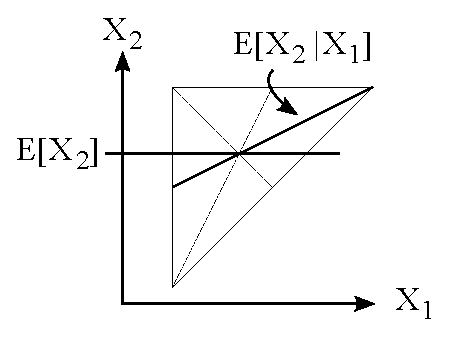
\includegraphics{Images/ConditionalExpectation.eps}
  \caption[Mean and Conditional Mean]
          {Mean and Conditional Mean}
  \label{fig:ConditionalExpectation}
\end{figure}

The probability density analog of the conditional probability statement is,

\begin{align*}
f_{X_2 | X_1 = x_1}(x_2) = \frac{f(x_1, x_2)}{f_{X_1}(x_1)}
\end{align*}

taking careful note of the upper-case (random variable) and lower-case (particular value). At this point we introduce some notational convenience,

\begin{align*}
f_1 &\equiv f_{X_1}\\
f_{2|1} &\equiv f_{X_2 | X_1 = x_1}
\end{align*}

To check that the conditional density function is valid we integrate it,

\begin{align*}
\int_{-\infty}^\infty f_{X_2 | X_1 = x_1}(x_2) \,\mathrm{d}x_2
&= \int_{-\infty}^\infty \frac{f(x_1, x_2)}{f_{X_1}(x_1)} \,\mathrm{d}x_2\\
&= \frac{1}{f_{X_1}(x_1)}\int_\mathbb{R} f(x_1, x_2) \,\mathrm{d}x_2\\
&= \frac{1}{f_{X_1}(x_1)}f_{X_1}(x_1)\\
&= 1
\end{align*}

Now we can define conditional expectation,

\begin{align*}
\mathbb{E} \left[X_2 | X_1 \right] 
&= \int_{-\infty}^\infty x_2 \, f_{X_2 | X_1}(x_2) \,\mathrm{d}x_2\\
&= \int_{-\infty}^\infty x_2 \, f_{2|1}(x_2) \,\mathrm{d}x_2 \in X_1
\end{align*}

where we emphasize that the result is a function of $X_1$. Recall that $\mathbb{E}[]$ is polymorphic and therefore it's meaning depends on context. The following should now be clear,

\begin{align}
\mathbb{E}\left[\mathbb{E}\left[X_2 | X_1 \right] \right]
&= \int_{-\infty}^\infty\int_{-\infty}^\infty x_2 \, f_{2|1}(x_2)\,\mathrm{d}x_2 f_1(x_1) \,\mathrm{d}x_1\\
&= \int_{-\infty}^\infty\int_{-\infty}^\infty x_2 \, f(x_1, x_2)\,\mathrm{d}x_2\mathrm{d}x_1\\
\label{eq:exp_exp} &= \mathbb{E}\left[X_2\right]
\end{align}

The figure \ref{fig:ConditionalExpectation} shows both the constant $\mathbb{E}[X_2]$ and the function of $X_1$, namely $\mathbb{E}[X_2 | X_1]$. Recall that the line $\mathbb{E}[X_2 | X_1]$ may not appear to resolve to $\mathbb{E}[X_1]$ on average, but it is a weighted average with, in the case of the figure, more weight associated with the left-most values of the line and less to the right-most values.

Now consider the conditional variance as it relates to unconditional variance. We start with the basics,

\begin{align}
\label{eq:var}      Var(X_2)       &= \mathbb{E}[X_2^2] - \mathbb{E}[X_2]^2\\
\label{eq:cond_var} Var(X_2 | X_1) &=  \mathbb{E}[X_2^2 | X_1] - \mathbb{E}[X_2 | X_1]^2
\end{align}

Now we do two things. We take the expectation of \ref{eq:cond_var},

\begin{align}
\mathbb{E}[Var(X_2 | X_1)] 
&= \mathbb{E}[\mathbb{E}[X_2^2 | X_1]] - \mathbb{E}[\mathbb{E}[X_2 | X_1]^2]\\
\label{eq:exp_cond} &= \mathbb{E}[X_2^2] - \mathbb{E}[\mathbb{E}[X_2 | X_1]^2]
\end{align}

then we find the variance of the conditional expectation,

\begin{align}
Var(\mathbb{E}[X_2 | X_1]) 
&= \mathbb{E}[\mathbb{E}[X_2 | X_1]^2] - \mathbb{E}[\mathbb{E}[X_2 | X_1]]\\
\label{eq:var_cond} &= \mathbb{E}[\mathbb{E}[X_2 | X_1]^2] - \mathbb{E}[X_2]^2
\end{align}

Noting that \ref{eq:var} =  \ref{eq:exp_cond} + \ref{eq:var_cond} we find our main result,

\begin{align}
\boxed{
Var(X_2) = \mathbb{E}[Var(X_2 | X_1)] + Var(\mathbb{E}[X_2 | X_1])
}
\end{align}

Our take-away is that, on average, the variance of a conditioned variable tends to be less that the variance of that same variable, unconditioned. Referring to figure \ref{fig:ConditionalExpectation} our physical analog is that the rotational inertia of the triangle is less than the $\mathbb{E}[X_2 | X_1]$ line. The difference is the average rotational inertia along the $\mathbb{E}[X_2 | X_1]$ line.


%%%%%%%%%%%%%%%%%%%%%%%%%%%%%%%%%%%%%%%%%%%%%%%%%%%%%%%%%%%%%%%%%%%%%%%%%%%%%%%%%%%%%%%%%%
\bibliographystyle{plain}
\bibliography{RticPHoX}
%%%%%%%%%%%%%%%%%%%%%%%%%%%%%%%%%%%%%%%%%%%%%%%%%%%%%%%%%%%%%%%%%%%%%%%%%%%%%%%%%%%%%%%%%%
\end {document}
